\documentclass{beamer}
\usepackage[utf8]{inputenc}
\usepackage{graphicx}
\usepackage{color}
%\usetheme{Hannover}
\newcommand{\hilight}[1]{\textbf{\textcolor{structure.fg!85}{#1}}}
\setbeamertemplate{footline}[frame number]

\usepackage{hyperref}
\hypersetup{
    colorlinks=true,
    linkcolor=blue,
    filecolor=magenta,      
    urlcolor=cyan,
}

\author[Sowmya Vajjala]{Sowmya Vajjala}

\title[SfSNLP]{NLP without Annotated Dataset}
\subtitle{NLP for Endangered Languages}


\date{27 January 2021}

\institute{Seminar f\"ur Sprachwissenschaft, University of T\"ubingen, Germany}
%%%%%%%%%%%%%%%%%%%%%%%%%%%

\begin{document}

\begin{frame}\titlepage
\end{frame}

\begin{frame}{}
    \Large Why is this topic of interest to anyone?
\end{frame}

\begin{frame}{What is different?}
Isn't it just NLP with another new language? a case of multilingual NLP? \pause
    \begin{itemize}
        \item What is needed? can be different 
        \item What is possible? can be different.
        \item Why is it needed? can be different.
    \end{itemize}
\end{frame}

\begin{frame}{What are some goals?}
    \begin{itemize}
        \item Language documentation
        \item Language preservation
        \item Enabling communication (e.g., typing on phone)
        \item May be support teaching/learning of that language
    \end{itemize}
\end{frame}

\begin{frame}{}
    "Systems constructed with zero expert resources [can] help
field linguists document endangered languages, by providing
tools to semi-automatically analyze and annotate audio
recordings using automatically discovered linguistic units”

–Dunbar et al. (2017) The Zero Resource Speech Challenge
2017. Proc IEEE ASRU Workshop.

\href{https://www.aclweb.org/anthology/2020.coling-main.313/}{Source}
\end{frame}

\begin{frame}{What kind of stuff is useful?}
\framesubtitle{Speech Technologies}
    \begin{itemize}
        \item There may be several hours of audio recordings sometimes, for some language groups (due to field linguists efforts, community recordings etc.)
        \item However, accessing them like a human being can be difficult (how to search through them? are they transcribed? what languages are being spoken? etc) \pause
        \item What is needed: Tools that can transcribe speech/label it/make it searchable somehow.
    \end{itemize}
\end{frame}

\begin{frame}{What kind of stuff is useful?}
\framesubtitle{Text Technologies}
    \begin{itemize}
    \item Typically, a lot of languages are morphologically complex, and current NLP methods may not exactly work
    \item So, from seemingly simple stuff like writing/speaking tools to grammar/spell checkers - everything can be much more challenging. 
    \end{itemize}
\end{frame}

\begin{frame}{Where is NLP research connecting to this?}
    \begin{itemize}
        \item Mobile applications for data collection related to language documentation (e.g., \href{https://www.aclweb.org/anthology/W17-0121/}{Bettinson \& Bird, 2017}
        \item Speech to text tools for field linguists (and others) (e.g., \href{https://isca-speech.org/archive/Interspeech_2019/pdfs/8006.pdf}{Foley et.al., (2019)} tested this for Abui, an Indonesian language with 17000 speakers)
        \item Machine Translation and language revitalization \href{https://www.aclweb.org/anthology/2020.coling-main.410/}{Le and Sadat, 2020}
        \item Developing language resources such as Universal Dependencies treebanks (https://universaldependencies.org/) 
    \end{itemize}
    ... ... ...
\end{frame}

\begin{frame}{}
    \Large Some current research projects
\end{frame}

\begin{frame}{Projects at my organization (NRC, Canada)}
    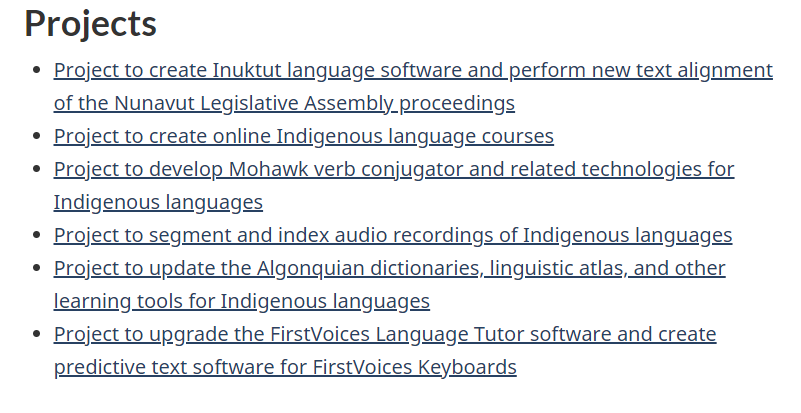
\includegraphics[width=\textwidth]{figures/ILT.PNG}
    
    (note: I am not involved with these. I can find out details if any of you are interested. )
\end{frame}

\begin{frame}{Text Input tools}
    \framesubtitle{\href{https://www.aclweb.org/anthology/2020.coling-main.405/}{"Interactive Word Completion for Morphologically Complex Languages"}}
    \begin{itemize}
        \item developed a method for morphologically-aware text input in Kunwinjku, a polysynthetic language of
northern Australia. 
        \item tested its portability through a relatively more known morphologically complex language - Turkish.
        \item deployed it as a usable tool and reported on its use. 
    \end{itemize}
    
    \textit{Lane, W., \& Bird, S. (2020, December). Interactive Word Completion for Morphologically Complex Languages. In Proceedings of the 28th International Conference on Computational Linguistics (pp. 4600-4611).}
    
    Note: Other efforts of this kind exist for other languages. 
\end{frame}

\begin{frame}{Speech Transcription tools}
\framesubtitle{\href{https://www.aclweb.org/anthology/2020.coling-main.303/}{"Enabling Interactive Transcription in an Indigenous Community"}}
    \begin{itemize}
        \item Focus on Kunwinjku- Language spoken by ~1500 people
        \item Task: speech transcription
        \item Result: Early stage deployment
        \item No training required.
        \item Participation of Indigenous people in the transcription process
    \end{itemize}
    
\textit{Le Ferrand, E., Bird, S., \& Besacier, L. (2020, December). Enabling Interactive Transcription in an Indigenous Community. In Proceedings of the 28th International Conference on Computational Linguistics (pp. 3422-3428).}

Note: Other efforts of this kind exist for other languages. 
\end{frame}

\begin{frame}{Other tools}
\framesubtitle{\href{https://www.aclweb.org/anthology/2020.lrec-1.345/}{"Learnings from Technological Interventions in a Low Resource Language: A Case-Study on Gondi"}}

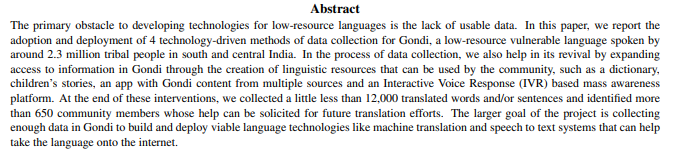
\includegraphics[width=\textwidth]{figures/gondi.PNG}
    
    \textit{Mehta, D., et.al. (2020, May). Learnings from Technological Interventions in a Low Resource Language: A Case-Study on Gondi. In Proceedings of The 12th Language Resources and Evaluation Conference (pp. 2832-2838).}
\end{frame}

\begin{frame}{However ....}
\framesubtitle{\href{https://www.aclweb.org/anthology/2020.acl-main.560/}{"The State and Fate of Linguistic Diversity and Inclusion in the NLP World"}}
    \begin{itemize}
        \item There are still a lot of languages in the world without any sort of NLP support.
        \item We still don't know much about how "language agnostic" are our language agnostic technologies. 
    \end{itemize}
    
\textit{Joshi, P., Santy, S., Budhiraja, A., Bali, K., \& Choudhury, M. (2020, July). The State and Fate of Linguistic Diversity and Inclusion in the NLP World. In Proceedings of the 58th Annual Meeting of the Association for Computational Linguistics (pp. 6282-6293).}
\end{frame}

\begin{frame}{Some Caveats}
It is more than "doing NLP on another new language".
    \begin{itemize}
            \item "The research must be done respectfully, in collaboration with the communities who
are the custodians of these languages. There should be no room in this field for scholars whose main goal is extracting “interesting” research without considering the linguistic needs of communities" \href{https://www.aclweb.org/anthology/2020.coling-main.516.pdf}{(Kuhn et.al., COLING 2020)}
        \item "While working with well-resourced languages, the main problem in designing language technologies is engineering. For low-resource languages, however, the main problem is one of designing methods for data collection upon which the language technology can be built." (Mehta et.al., 2020) \pause
    \end{itemize}
\end{frame}

\begin{frame}{Getting Started}
    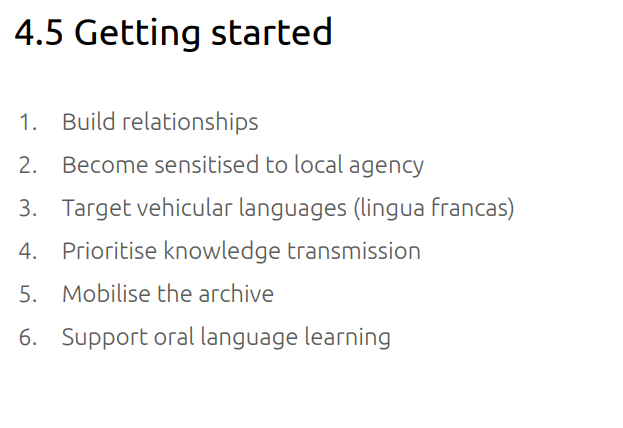
\includegraphics[width=\textwidth]{figures/gettingstarted-bird.PNG}
\end{frame}

\begin{frame}{Resources to explore further}
    \begin{itemize}
        \item \href{https://spectrum.library.concordia.ca/986506/7/Indigenous_Protocol_and_AI_2020.pdf}{Indigenous Protocol and AI - position paper}
        \item \href{https://github.com/neubig/lowresource-nlp-bootcamp-2020}{CMU's low resource NLP bootcamp, 2020}
        \item \href{https://nrc.canada.ca/en/research-development/research-collaboration/programs/canadian-indigenous-languages-technology-project}{Indigenous Language Technologies project}
        \item \url{https://github.com/LowResourceLanguages/}
        \item \href{https://computel-workshop.org/}{Workshops on the use of Computational Methods in the Study of Endangered Languages}
    \item \href{https://www.aclweb.org/anthology/2020.coling-tutorials.7.pdf}{Reading List on NLP for Endangered Languages} (scroll to the end to see the list)
     \item \href{https://scholar.google.com/citations?user=xoyloJAAAAAJ&hl=en&oi=ao}{Follow work by Steven Bird (a co-author of NLTK/NLTK book)}
    \end{itemize}
\end{frame}

\begin{frame}{To get a taste of it}
Do the first part of the exercise described in Chintang.pdf :-) It is from NACLO, again. 
    
\end{frame}

\end{document}